% Volume II: Calculus, Analysis, and Continuous Mathematics
% Continuity note for Chapter 11.
% Previous dependencies: Chapters 1-2 introduced typed objects, sets, functions, domains, codomains, and inverse images; Chapters 3-5 supplied geometric language for vectors, volume intuition, projections, and coordinates; Chapters 8-9 introduced integrals, multivariable domains, Jacobians, and local linear maps; Chapter 10 motivates curved coordinate systems and constrained surfaces that require coordinate-aware integration.
% New durable concepts: measurable spaces; sigma-algebras; measures; probability measures; null sets; almost-everywhere reasoning; measurable functions; Lebesgue-style integration by simple functions; densities with respect to base measures; high-dimensional integrals, marginalization, and Monte Carlo estimation; change of variables with Jacobian determinants; Dirac measures, delta notation, test functions, generalized functions, and impulse convolution.
% Forward hooks: Chapter 12 reuses integration and almost-everywhere equality for L^2 function spaces; Chapter 13 reuses measurable spaces and random variables as measurable functions; Chapters 14-15 reuse densities, expectations, conditioning, and atoms; Chapters 17-18 reuse likelihood integrals, KL integrals, and Fisher geometry; later ML chapters reuse change of variables for normalizing flows, variational inference, latent-variable models, and neural population distributions.
% Notation commitments: measurable spaces are written (\Omega,\mathcal{F}); measures are \mu, Lebesgue measure is \lambda, and probability measures are P; measurable sets are A,B,E; null sets are N; densities are p or q with respect to dx or a base measure \mu; expectations are \mathbb{E}[g(X)]; transformations are T:U\to V with Jacobian J_T(x); Dirac point masses are \delta_a, and test functions are \varphi.
% Figure plan: four ImageGen raster figures under imagegen-figures/ch11-* are referenced: measurable spaces and measure integration for 11.1; densities, marginalization, grids, and Monte Carlo for 11.2; Jacobian change of variables for 11.3; delta functions and impulse responses for 11.4.
\section{Chapter 11: Measure, Integration, and Change of Variables}
\label{ch:measure-integration-change-variables}

Chapters 8-10 made continuous mathematics local and geometric. Derivatives were local linear maps. Hessians described local curvature. Manifolds were spaces that look flat when viewed through a good coordinate chart. But continuous models also require another operation: adding contributions over a space. A probability density must integrate to one. A likelihood averages over latent variables. A neural population model assigns probability to regions of response space, not only to single observed vectors.

Ordinary finite sums are not enough for those tasks. In a continuous space, a single point usually has zero volume, yet regions can have positive probability. Some sets are so irregular that assigning them a consistent size breaks the rules we want size to obey. Some useful objects, such as ideal point masses and spike impulses, are not ordinary finite-height functions at all. Measure theory is the language that makes these distinctions precise without losing the computational intuition.

\paragraph{Chapter problem.}
How can we assign size or probability to sets, integrate functions over high-dimensional spaces, and transform densities when coordinates change?

\paragraph{Section map.}
Section 11.1 explains why measure theory is needed and defines measurable spaces, measures, null sets, and almost-everywhere statements. Section 11.2 defines densities and high-dimensional integrals, including marginalization and Monte Carlo estimation. Section 11.3 derives the change-of-variables formula and the role of the Jacobian determinant. Section 11.4 treats delta functions as point masses and generalized functions, with spike trains and impulse responses as guiding examples.

\subsection{11.1 Why measure theory matters}

\paragraph{Motivating question.}
How can we assign size or probability to events in a way that remains consistent under complements, countable unions, and limiting operations?

\paragraph{Beginner setup.}
A \emph{measure} is a rule that assigns a nonnegative size to sets. Length on the real line, area in the plane, volume in \(\mathbb{R}^3\), counting size on a finite set, and probability are all measures. The point of measure theory is not to make integration abstract for its own sake. It is to say exactly which sets are allowed to receive sizes, and which rules those sizes must obey.

The smallest nontrivial example is a finite sample space
\[
\Omega=\{HH,HT,TH,TT\},
\]
the possible outcomes of tossing two fair coins. Let \(\mathcal{F}\) be the collection of all subsets of \(\Omega\). For any event \(A\subseteq\Omega\), define
\[
P(A)=\frac{|A|}{4}.
\]
If \(A=\{HH,HT\}\), then \(P(A)=2/4=1/2\). If \(B=\{HH\}\), then \(P(B)=1/4\). The empty event has probability \(0\), and the whole space has probability \(1\).

The continuous example is length on intervals. If \(A=[0,2]\), then its length is \(2\). If \(B=[1,4]\), then its length is \(3\). A single point, such as \(\{2\}\), has length \(0\), even though it is not empty. This is the first sign that continuous size behaves differently from finite counting.

What to keep in mind: measure theory separates three objects that beginners often merge. There is an underlying space \(\Omega\). There is a collection \(\mathcal{F}\) of measurable sets whose sizes we are allowed to discuss. There is a measure \(\mu\) that assigns sizes to those measurable sets.

\begin{figure}[htbp]
\centering
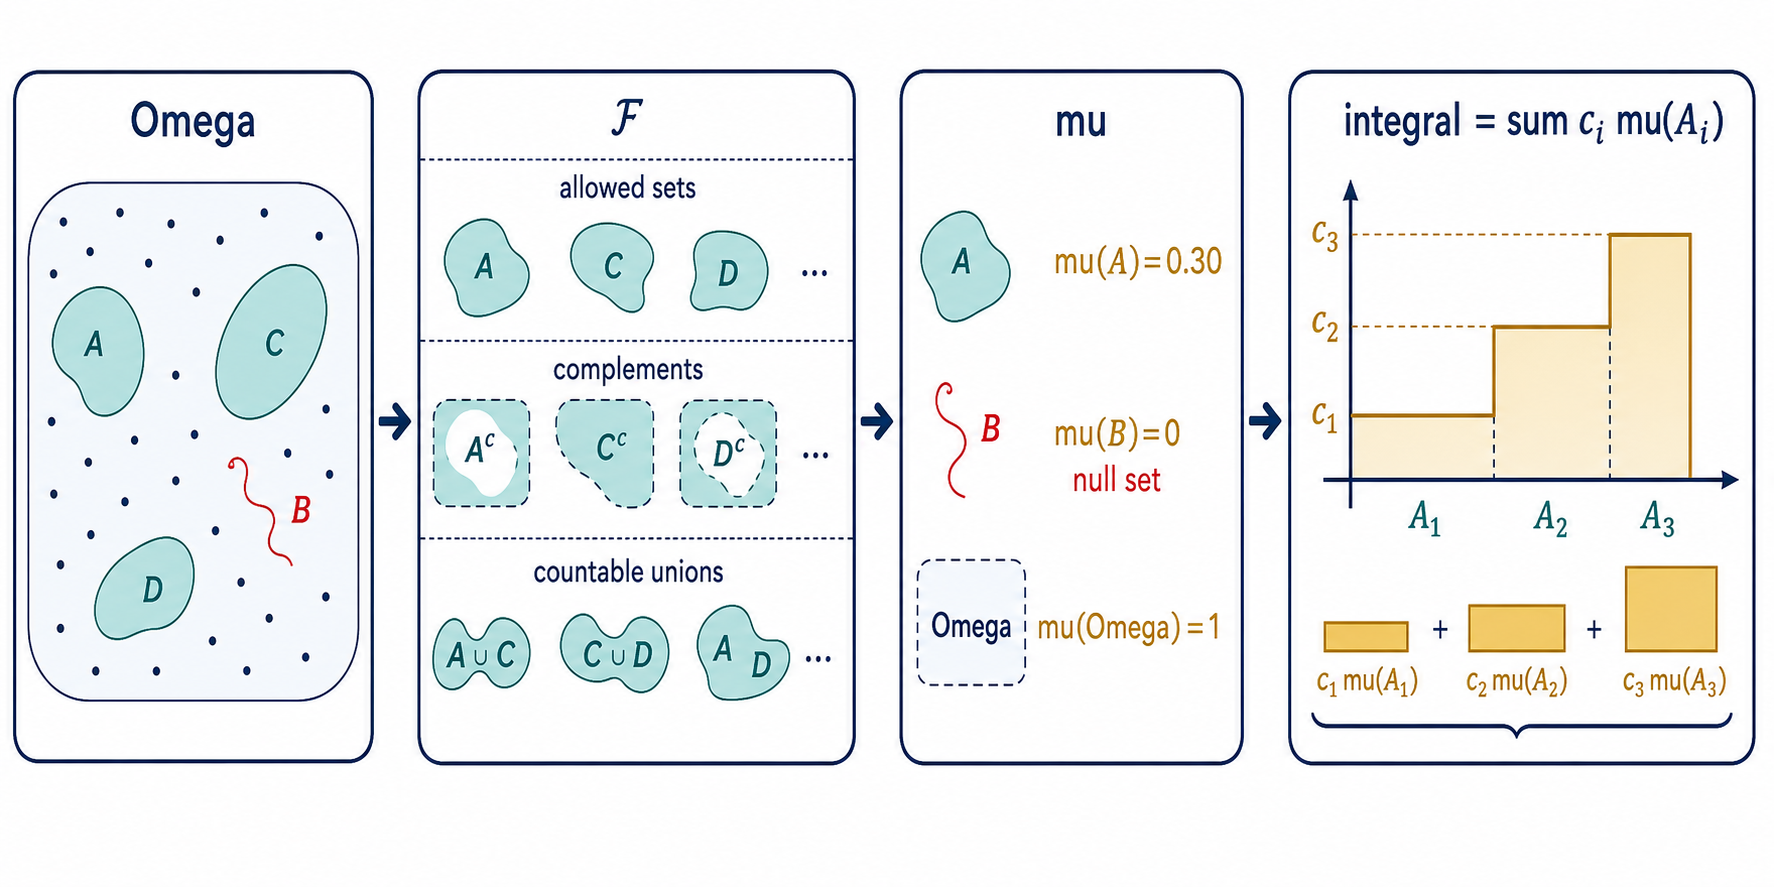
\includegraphics[width=0.98\linewidth]{imagegen-figures/ch11-measure-space-integration.png}
\caption{A measure-theoretic model has three layers: the space \(\Omega\), the allowed measurable sets \(\mathcal{F}\), and a measure \(\mu\) assigning consistent sizes to those sets. Integrals are built by adding function levels over measurable pieces, first for simple functions and then by limits. Null sets have measure zero even when they are not empty.}
\label{fig:ch11-measure-space-integration}
\end{figure}

\paragraph{Formal setup.}
A \emph{measurable space} is a pair
\[
(\Omega,\mathcal{F}),
\]
where \(\Omega\) is a set and \(\mathcal{F}\) is a \(\sigma\)-algebra of subsets of \(\Omega\). This means:
\[
\Omega\in\mathcal{F},\qquad
A\in\mathcal{F}\Longrightarrow A^c\in\mathcal{F},\qquad
A_1,A_2,\ldots\in\mathcal{F}\Longrightarrow \bigcup_{i=1}^{\infty} A_i\in\mathcal{F}.
\]
Closure under complements and countable unions also gives closure under countable intersections, because
\[
\bigcap_{i=1}^{\infty} A_i
=\left(\bigcup_{i=1}^{\infty} A_i^c\right)^c.
\]

A \emph{measure} on \((\Omega,\mathcal{F})\) is a function
\[
\mu:\mathcal{F}\to[0,\infty]
\]
such that
\[
\mu(\emptyset)=0
\]
and, whenever \(A_1,A_2,\ldots\) are pairwise disjoint measurable sets,
\[
\mu\!\left(\bigcup_{i=1}^{\infty}A_i\right)
=
\sum_{i=1}^{\infty}\mu(A_i).
\]
This countable additivity equation is the central rule. It says that the size of a disjoint union is the sum of the sizes, even for countably many pieces.

A \emph{probability measure} is a measure \(P\) with
\[
P(\Omega)=1.
\]
A \emph{null set} is a measurable set \(N\) with \(\mu(N)=0\). A statement holds \emph{almost everywhere} if it may fail on a null set but holds outside that set. A function \(f:\Omega\to\mathbb{R}\) is \emph{measurable} if sets of the form
\[
\{\omega\in\Omega:f(\omega)\leq t\}
\]
belong to \(\mathcal{F}\) for every real threshold \(t\). This condition ensures that questions about the function's values define measurable events.

Integration starts with simple measurable functions. If
\[
s(\omega)=\sum_{i=1}^n c_i\mathbf{1}_{A_i}(\omega),
\]
where \(A_i\in\mathcal{F}\), \(c_i\geq0\), and the \(A_i\) are disjoint, then
\[
\int_\Omega s\,d\mu
=
\sum_{i=1}^n c_i\mu(A_i).
\]
General nonnegative integrals are obtained by approximating from below with such simple functions; integrable signed functions are handled by separating positive and negative parts when both accumulated sizes are finite. This is the formal version of adding weighted measurable pieces.

\paragraph{Core intuition.}
Figure~\ref{fig:ch11-measure-space-integration} shows the bookkeeping role of \(\mathcal{F}\). The \(\sigma\)-algebra is the collection of questions about \(\Omega\) that the model agrees are meaningful. If \(A\) is meaningful, then "not \(A\)" should also be meaningful. If each \(A_i\) is meaningful, then "at least one of these \(A_i\) occurs" should be meaningful. This closure is why countable unions and complements appear in the definition.

The measure \(\mu\) is not the same thing as the set. It is a size assigned to the set. On a finite space, measure may look like counting. On \(\mathbb{R}\), Lebesgue measure behaves like length. In probability, the measure is not physical size but probability mass.

The most important continuous-space surprise is that nonempty sets can have measure zero. A single time point has zero length. A single exact neural response vector usually has zero volume in a continuous response model. That does not mean the point is impossible as a mathematical input; it means probability must be assigned to regions or represented by other objects such as point masses.

A common misconception is that every subset should be measurable. For most practical ML and neuroscience work, standard sets such as intervals, rectangles, balls, level sets of continuous functions, and countable unions of these are measurable. But insisting that every imaginable subset of \(\mathbb{R}\) receive a length while preserving translation invariance and countable additivity leads to contradictions. Measure theory handles this by specifying the allowed sets.

This section reuses Chapter 2's discipline about domains and inverse images. It prepares Chapter 13, where random variables will be measurable functions, and it prepares all later probability integrals.

\paragraph{Main theorem: basic bookkeeping laws of measure.}
Let \((\Omega,\mathcal{F},\mu)\) be a measure space.

\emph{Finite additivity.} If \(A_1,\ldots,A_n\in\mathcal{F}\) are pairwise disjoint, then
\[
\mu\!\left(\bigcup_{i=1}^n A_i\right)
=\sum_{i=1}^n\mu(A_i).
\]

\emph{Monotonicity.} If \(A,B\in\mathcal{F}\) and \(A\subseteq B\), then
\[
\mu(A)\leq \mu(B).
\]

\emph{Proof sketch.}
Finite additivity is countable additivity with all later sets empty:
\[
A_{n+1}=A_{n+2}=\cdots=\emptyset.
\]
Because \(\mu(\emptyset)=0\), the infinite sum reduces to the finite sum.

For monotonicity, write \(B\) as the disjoint union
\[
B=A\cup(B\setminus A).
\]
Both sets are measurable because \(\mathcal{F}\) is closed under complements and intersections. Finite additivity gives
\[
\mu(B)=\mu(A)+\mu(B\setminus A).
\]
Since measures are nonnegative, \(\mu(B\setminus A)\geq0\), so \(\mu(B)\geq\mu(A)\). The algebra is simple, but the mechanism matters: measure laws are consequences of countable additivity plus closure of the allowed sets.

\paragraph{Worked examples.}
\emph{Small finite example.} Let \(\Omega=\{1,2,3,4,5,6\}\), let \(\mathcal{F}\) be all subsets, and define \(P(A)=|A|/6\). If
\[
A=\{2,4,6\},\qquad B=\{1,3\},
\]
then \(A\cap B=\emptyset\), so
\[
P(A\cup B)=P(A)+P(B)=\frac{3}{6}+\frac{2}{6}=\frac{5}{6}.
\]
The complement of \(A\) is \(A^c=\{1,3,5\}\), and \(P(A^c)=1-P(A)=1/2\).

\emph{ML/neuroscience example.} In a spike-count experiment, \(\Omega\) might be all possible spike-count sequences over a trial. The event
\[
A=\{\text{the neuron fires at least five spikes in the first }100\text{ ms}\}
\]
is a measurable subset of \(\Omega\). A probability measure \(P\) assigns \(P(A)\), the probability of that event under a stimulus condition. If responses are modeled continuously, such as \(X\in\mathbb{R}^{100}\) for a population activity vector, the exact event \(\{X=x_0\}\) often has probability zero, while a ball \(\{x:\|x-x_0\|_2\leq r\}\) can have positive probability. The model therefore predicts probabilities of neighborhoods or decision regions, not usually exact continuous vectors.

\paragraph{ML/DL/neuroscience connections.}
In probability, \(\Omega\) becomes the sample space of possible outcomes, \(\mathcal{F}\) becomes the event system, and \(P\) becomes uncertainty. In supervised learning, events may be subsets of data-label pairs \((x,y)\). In latent-variable models, events may involve both observed variables \(x\) and hidden variables \(z\). In neuroscience, measurable events can be spike-count ranges, stimulus categories, reaction-time intervals, or regions of neural state space. Null sets justify almost-everywhere statements: two density formulas may differ at a few points and still define the same continuous probability law.

\paragraph{Exercises.}
\begin{enumerate}[label=\textbf{11.1.\arabic*.}, leftmargin=*]
\item \textbf{Mechanical.} Let \(\Omega=\{a,b,c,d\}\), \(\mathcal{F}=2^\Omega\), and \(\mu(A)=2|A|\). Compute \(\mu(\Omega)\), \(\mu(\{a,c\})\), and \(\mu(\emptyset)\).
\item \textbf{Proof or derivation.} Prove that if \(A\subseteq B\) and \(\mu(A)<\infty\), then \(\mu(B\setminus A)=\mu(B)-\mu(A)\).
\item \textbf{Numerical/computational.} Suppose a dataset has \(1000\) trials and \(73\) trials contain at least one spike in a chosen time bin. Treating empirical frequency as a probability measure on trials, estimate the measure of that event.
\item \textbf{Interpretation.} In a continuous model for \(X\in\mathbb{R}^d\), why can \(P(X=x_0)=0\) while observations near \(x_0\) are still common?
\item \textbf{Debug the misconception.} A student says, "A null set is the same as the empty set." Explain the difference using a point in \(\mathbb{R}\) with length measure.
\end{enumerate}

\subsection{11.2 Densities and integration in high dimensions}

\paragraph{Motivating question.}
How do we compute probability, averages, and marginal distributions when outcomes live in a high-dimensional continuous space?

\paragraph{Beginner setup.}
A \emph{density} is not the probability of a point. It is probability per unit volume. For a continuous random vector \(X\in\mathbb{R}^d\), a density \(p\) satisfies
\[
p(x)\geq0,
\qquad
\int_{\mathbb{R}^d}p(x)\,dx=1.
\]
The probability of a region \(A\subseteq\mathbb{R}^d\) is
\[
P(X\in A)=\int_A p(x)\,dx.
\]

The smallest nontrivial example is the uniform density on the interval \([0,2]\):
\[
p(x)=
\begin{cases}
1/2, & 0\leq x\leq2,\\
0, & \text{otherwise}.
\end{cases}
\]
The probability of the region \([0.5,1.5]\) is
\[
\int_{0.5}^{1.5}\frac{1}{2}\,dx=\frac{1}{2}.
\]
No single point has positive probability, but intervals do.

In high dimensions, the same idea holds, but direct grids become expensive. If each coordinate is evaluated at \(m\) grid locations, then a \(d\)-dimensional grid has \(m^d\) points. With \(m=100\) and \(d=10\), this is \(100^{10}=10^{20}\) grid points. This is why high-dimensional integration usually relies on structure, approximation, factorization, variational methods, or Monte Carlo samples.

What to keep in mind: a density becomes a probability only after being integrated over a measurable set. In high dimensions, most of the work is choosing a representation or estimator that avoids enumerating every tiny cell.

\begin{figure}[htbp]
\centering
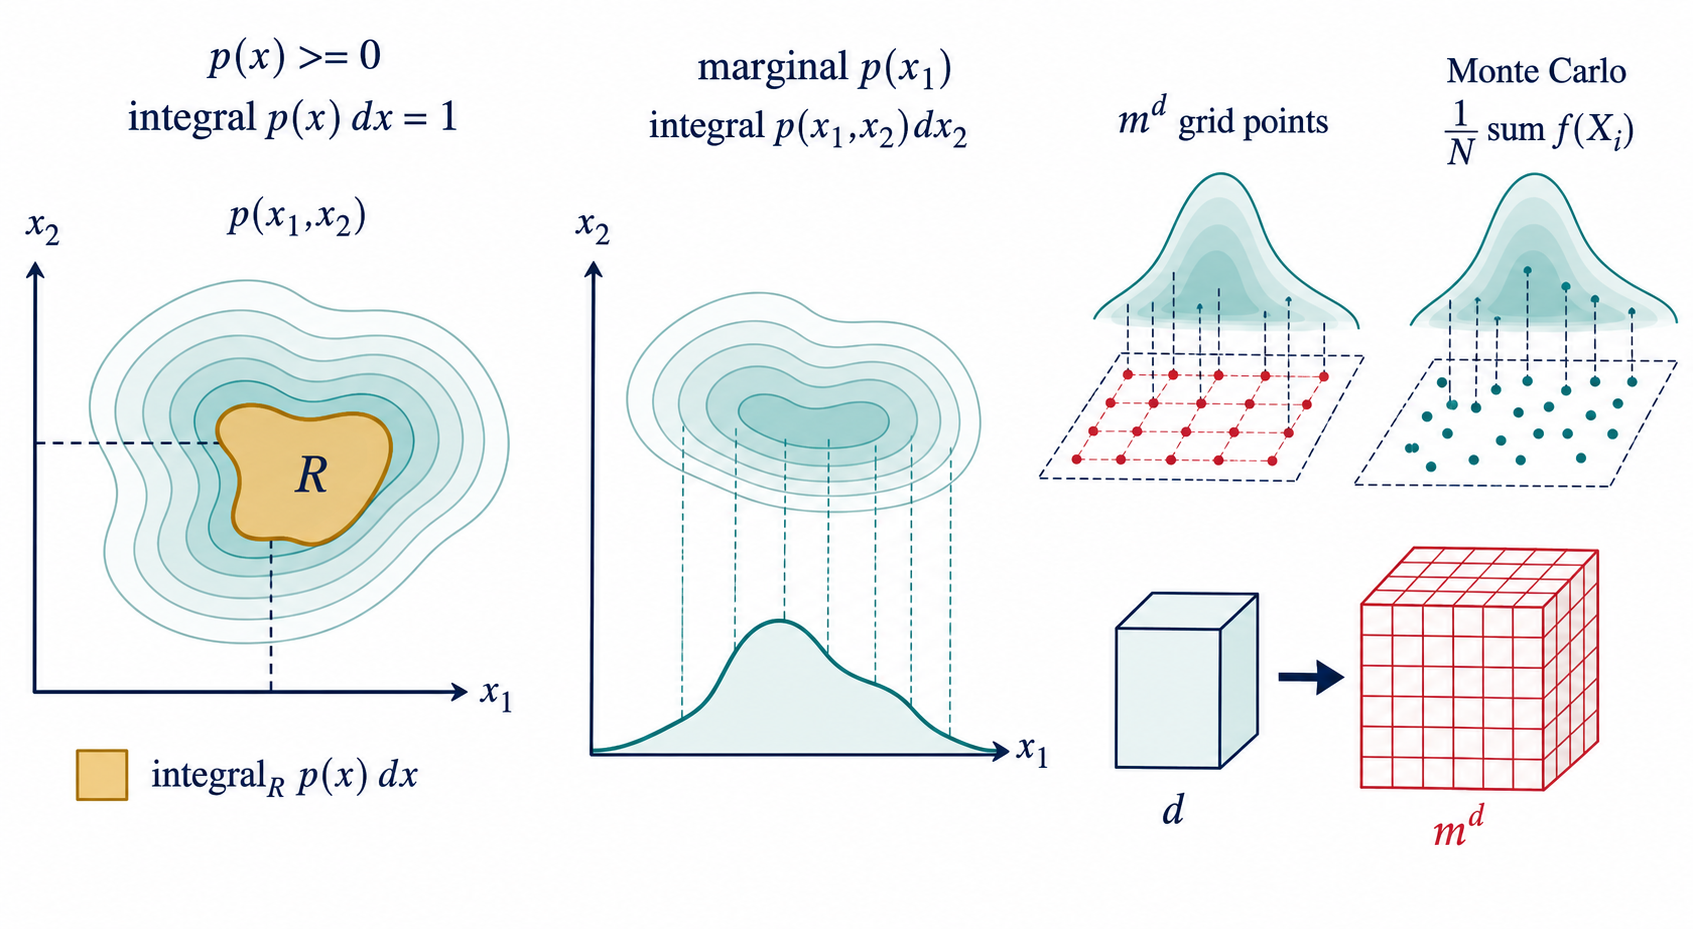
\includegraphics[width=0.98\linewidth]{imagegen-figures/ch11-densities-high-dim-integration.png}
\caption{A density assigns probability per unit volume. Region probabilities are integrals under the density, marginal densities are obtained by integrating out coordinates, and high-dimensional grid integration grows like \(m^d\). Monte Carlo replaces a full grid by random samples and estimates expectations with sample averages.}
\label{fig:ch11-densities-high-dim-integration}
\end{figure}

\paragraph{Formal setup.}
Let \(X\) be a random vector in \(\mathbb{R}^d\). A density \(p_X:\mathbb{R}^d\to[0,\infty)\) with respect to Lebesgue measure \(dx\) represents the probability measure \(P_X\) by
\[
P_X(A)=\int_A p_X(x)\,dx
\]
for measurable \(A\subseteq\mathbb{R}^d\). The normalization condition is
\[
\int_{\mathbb{R}^d}p_X(x)\,dx=1.
\]
For an integrable function \(g:\mathbb{R}^d\to\mathbb{R}\), expectation is
\[
\mathbb{E}[g(X)]
=
\int_{\mathbb{R}^d}g(x)p_X(x)\,dx.
\]

If \(X=(U,V)\), where \(U\in\mathbb{R}^k\) and \(V\in\mathbb{R}^{d-k}\), and the joint density is \(p_{U,V}(u,v)\), then the marginal density of \(U\) is
\[
p_U(u)=\int_{\mathbb{R}^{d-k}}p_{U,V}(u,v)\,dv.
\]
This equation is the continuous analogue of summing a joint probability table over the variables we do not keep.

If \(X_1,\ldots,X_N\) are independent samples from \(p_X\), the Monte Carlo estimator for \(\mathbb{E}[g(X)]\) is
\[
\widehat{I}_N=\frac{1}{N}\sum_{i=1}^N g(X_i).
\]
Its accuracy depends on variance and sample size, not directly on a full \(m^d\) grid.

\paragraph{Core intuition.}
Figure~\ref{fig:ch11-densities-high-dim-integration} connects three operations. Integrating over a region adds up density times tiny volumes inside that region. Marginalizing removes coordinates by integrating over them. Monte Carlo integration replaces an exhaustive grid by representative random draws.

High-dimensional geometry is unintuitive because volume spreads out. A small interval covers a visible fraction of a line, but a small box covers a tiny fraction of a high-dimensional cube. As a simplifying illustration, suppose the coordinate events are independent and each coordinate has probability \(0.9\) of lying in its central range. Then all \(d\) coordinates lie in their central ranges with probability \(0.9^d\), which decays quickly. Without the independence assumption, the exact probability need not equal \(0.9^d\), but the example shows why high-dimensional central boxes can shrink in probability very fast.

A common misconception is to read \(p(x)\) as \(P(X=x)\). For continuous densities, \(P(X=x)=0\) for each fixed point under ordinary Lebesgue densities. The density may be large at \(x\), but probability comes from a region around \(x\). Another misconception is that higher density always means higher probability for any nearby set. The size and shape of the set also matter.

This section extends Chapter 8's integrals from accumulated one-dimensional quantities to high-dimensional probability and expectation. It prepares probability spaces, distributions, Bayesian marginalization, likelihoods, and information integrals.

\paragraph{Main derivation: marginalization and unbiased Monte Carlo.}
Suppose \(p_{U,V}(u,v)\) is a joint density normalized on \(\mathbb{R}^k\times\mathbb{R}^{d-k}\). Define
\[
p_U(u)=\int p_{U,V}(u,v)\,dv.
\]
Then \(p_U\) is normalized:
\[
\int p_U(u)\,du
=
\int\left(\int p_{U,V}(u,v)\,dv\right)du
=
\int\int p_{U,V}(u,v)\,dv\,du
=1,
\]
where the interchange and repeated integration are justified under the usual nonnegativity or integrability conditions. The mechanism is the same as summing rows or columns of a probability table: all probability mass is retained, but the \(v\)-coordinate is no longer reported.

For Monte Carlo, let \(X_1,\ldots,X_N\) be independent samples from \(p_X\), and let \(g(X)\) have finite expectation. Then
\[
\mathbb{E}[\widehat{I}_N]
=
\mathbb{E}\left[\frac{1}{N}\sum_{i=1}^N g(X_i)\right]
=
\frac{1}{N}\sum_{i=1}^N\mathbb{E}[g(X_i)]
=
\mathbb{E}[g(X)].
\]
Thus the sample average is an unbiased estimator of the desired integral. Variance controls how many samples are needed for a stable estimate.

\paragraph{Worked examples.}
\emph{Small numerical example.} Let
\[
p(x,y)=4xy,\qquad 0\leq x\leq1,\quad 0\leq y\leq1,
\]
and \(p(x,y)=0\) otherwise. It is normalized because
\[
\int_0^1\int_0^1 4xy\,dy\,dx
=
4\left(\int_0^1 x\,dx\right)\left(\int_0^1 y\,dy\right)
=4\cdot\frac{1}{2}\cdot\frac{1}{2}=1.
\]
The probability of the rectangle \(R=\{x>1/2,\ y<1/2\}\) is
\[
\int_{1/2}^{1}\int_0^{1/2}4xy\,dy\,dx
=
4\left(\frac{1^2-(1/2)^2}{2}\right)\left(\frac{(1/2)^2}{2}\right)
=\frac{3}{16}.
\]
The marginal density of \(X\) is
\[
p_X(x)=\int_0^1 4xy\,dy=2x,\qquad 0\leq x\leq1.
\]

\emph{ML/neuroscience example.} In a latent-variable model, \(z\in\mathbb{R}^d\) might be an unobserved cause and \(x\) an observed neural response or image. The likelihood of \(x\) is often an integral
\[
p(x)=\int p(x\mid z)p(z)\,dz.
\]
Here \(p(z)\) is a density over latent states, \(p(x\mid z)\) is an observation model, and integrating over \(z\) marginalizes uncertainty about the hidden cause. In neural population analysis, \(x\in\mathbb{R}^{100}\) might be a vector of firing rates. A density \(p(x)\) describes how response vectors are distributed across trials, and an expectation \(\mathbb{E}[g(X)]\) can be an average decoder confidence, energy, or behavioral prediction over the population distribution.

\paragraph{ML/DL/neuroscience connections.}
In machine learning, the integral \(\int g(x)p(x)\,dx\) becomes expected loss, expected reward, or average feature value. In variational inference, difficult integrals over latent variables are replaced by lower bounds or Monte Carlo estimates under an approximate posterior \(q(z\mid x)\). In deep learning, minibatch training is a Monte Carlo estimate of population risk. In neuroscience, averaging a tuning-curve statistic over stimuli is an expectation, and marginalizing over nuisance variables such as eye position or adaptation state is an integral over hidden coordinates.

\paragraph{Exercises.}
\begin{enumerate}[label=\textbf{11.2.\arabic*.}, leftmargin=*]
\item \textbf{Mechanical.} Check that \(p(x)=3x^2\) on \([0,1]\) is normalized, and compute \(P(X>1/2)\).
\item \textbf{Proof or derivation.} Let \(p_{X,Y}(x,y)\) be a normalized nonnegative joint density. Derive \(p_X(x)=\int p_{X,Y}(x,y)\,dy\) and show that \(\int p_X(x)\,dx=1\).
\item \textbf{Numerical/computational.} A ten-dimensional grid uses \(50\) points per coordinate. How many grid points are required? If a Monte Carlo estimate uses \(10{,}000\) samples instead, what tradeoff is being made?
\item \textbf{Interpretation.} Explain why a density value \(p(x_0)=10\) does not mean \(P(X=x_0)=10\), or even that \(P(X=x_0)\) is positive.
\item \textbf{Debug the misconception.} A student says, "Marginalizing over \(z\) throws away probability mass." Use the normalization derivation to explain why this is false.
\end{enumerate}

\subsection{11.3 Change of variables}

\paragraph{Motivating question.}
When a continuous variable is transformed by an invertible map, how must its density change so that probabilities of corresponding regions stay the same?

\paragraph{Beginner setup.}
A change of variables is a relabeling or transformation of the same underlying mass. If \(X\) is uniform on \([0,1]\) and
\[
Y=2X,
\]
then \(Y\) is uniform on \([0,2]\). The interval doubled in length, so the density must be cut in half:
\[
p_Y(y)=\frac{1}{2},\qquad 0\leq y\leq2.
\]
The probability mass is unchanged:
\[
P(0\leq X\leq 1)=1=P(0\leq Y\leq2).
\]

The general rule is the same. If a transformation stretches volume, density decreases. If it compresses volume, density increases. The Jacobian determinant measures that local volume scaling.

What to keep in mind: a density is tied to coordinates. Probability mass is invariant, but density values change when coordinates stretch or compress space.

\begin{figure}[htbp]
\centering
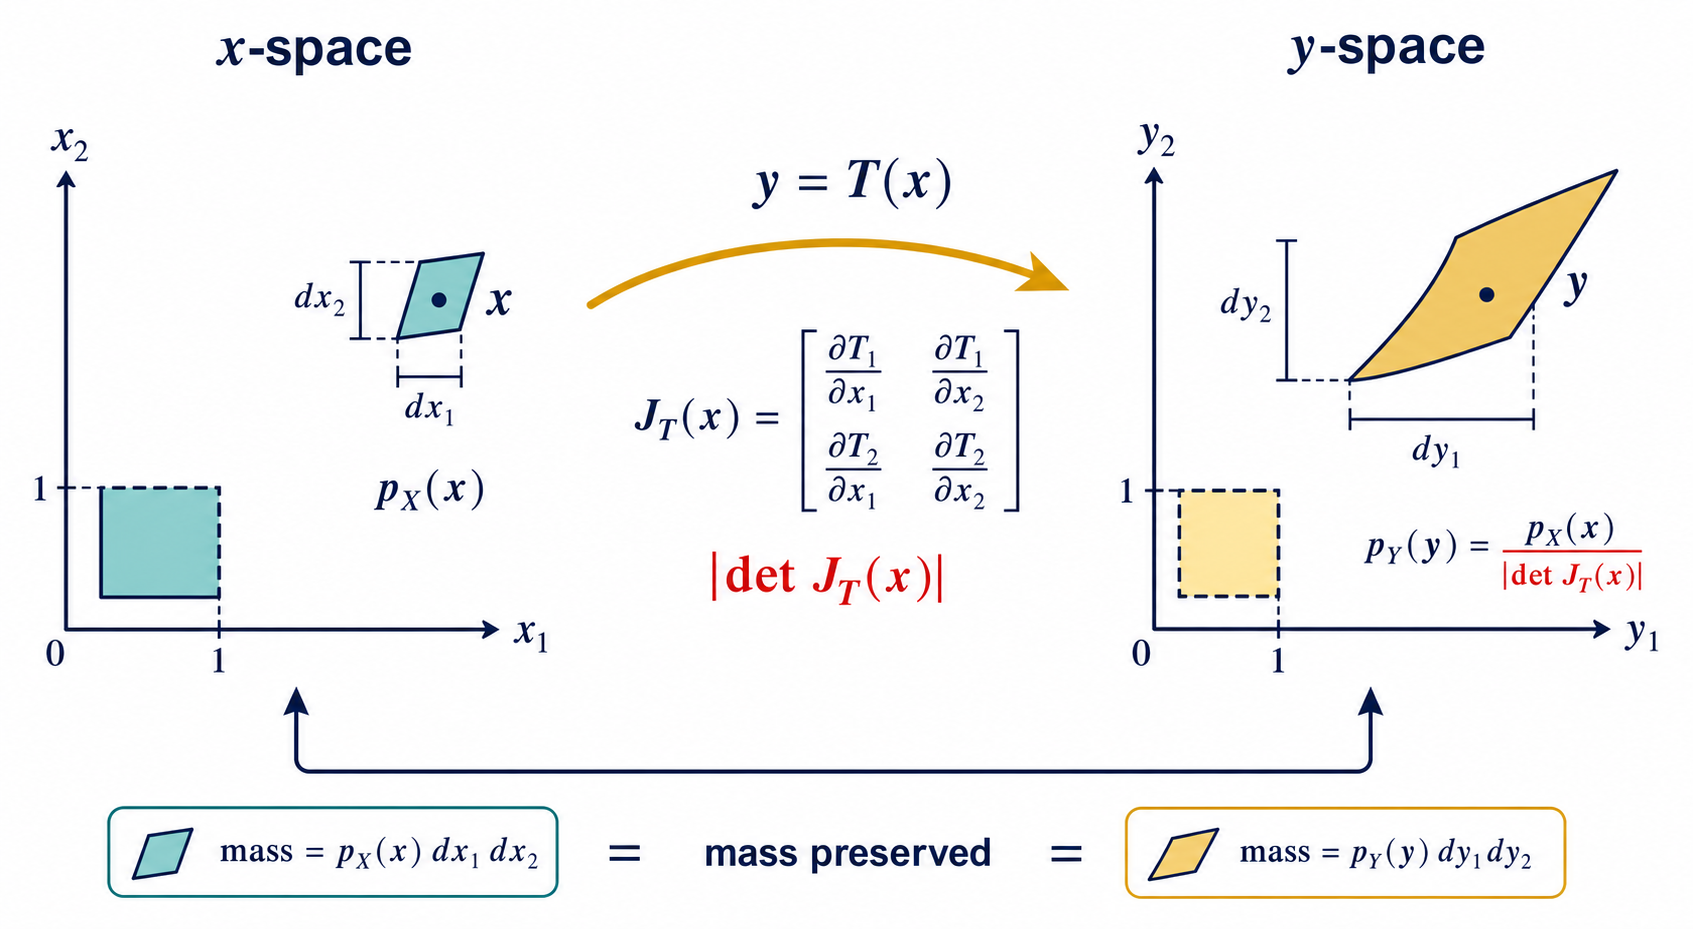
\includegraphics[width=0.98\linewidth]{imagegen-figures/ch11-change-of-variables-jacobian.png}
\caption{Under an invertible transformation \(y=T(x)\), a small input volume near \(x\) becomes a transformed volume near \(y\). The Jacobian determinant \(|\det J_T(x)|\) gives the local volume scale. Density changes inversely so that probability mass is preserved.}
\label{fig:ch11-change-of-variables-jacobian}
\end{figure}

\paragraph{Formal setup.}
Let \(U,V\subseteq\mathbb{R}^d\), and let
\[
T:U\to V
\]
be a continuously differentiable bijection with continuously differentiable inverse and nonzero Jacobian determinant. Write
\[
y=T(x),\qquad x=T^{-1}(y),
\]
and let
\[
J_T(x)=
\begin{bmatrix}
\dfrac{\partial T_1}{\partial x_1}(x) & \cdots & \dfrac{\partial T_1}{\partial x_d}(x)\\
\vdots & \ddots & \vdots\\
\dfrac{\partial T_d}{\partial x_1}(x) & \cdots & \dfrac{\partial T_d}{\partial x_d}(x)
\end{bmatrix}
\]
be the Jacobian matrix.

The integral change-of-variables formula is
\[
\int_V g(y)\,dy
=
\int_U g(T(x))\,|\det J_T(x)|\,dx.
\]
If \(X\) has density \(p_X\) on \(U\) and \(Y=T(X)\), then the density of \(Y\) is
\[
p_Y(y)
=
p_X(T^{-1}(y))\left|\det J_{T^{-1}}(y)\right|
=
\frac{p_X(x)}{|\det J_T(x)|},
\qquad y=T(x).
\]
The absolute value is required because density uses positive volume, not orientation.

\paragraph{Core intuition.}
Figure~\ref{fig:ch11-change-of-variables-jacobian} shows a small cell near \(x\). Locally, the nonlinear map \(T\) behaves like its Jacobian matrix \(J_T(x)\). From Chapter 4, a matrix maps small parallelepipeds to new parallelepipeds, and its determinant gives signed volume scaling. Taking the absolute value turns signed volume into ordinary volume.

The density formula is just conservation of mass:
\[
p_X(x)\,dx \approx p_Y(y)\,dy.
\]
Since
\[
dy\approx |\det J_T(x)|\,dx,
\]
we must have
\[
p_Y(y)\approx \frac{p_X(x)}{|\det J_T(x)|}.
\]
This is why stretching lowers density and compression raises density.

Common misconceptions are worth naming. The Jacobian determinant is not the same as the Jacobian matrix; it is a scalar volume factor extracted from the matrix. The absolute value matters. The formula requires local invertibility; if the map folds several \(x\)-values onto the same \(y\), their contributions must be summed over preimages. Finally, the formula transforms densities, not the underlying probability mass.

This section reuses Chapter 9's Jacobian as a local linear map and Chapter 10's coordinate-chart intuition. It is the mathematical core of normalizing flows and many coordinate transformations in statistics.

\paragraph{Main derivation: density transformation by mass preservation.}
Start in one dimension. Let \(T:\mathbb{R}\to\mathbb{R}\) be increasing and differentiable, and let \(Y=T(X)\). For a small interval \([x,x+\Delta x]\), the transformed interval has approximate length
\[
\Delta y\approx T'(x)\Delta x.
\]
Mass preservation gives
\[
p_X(x)\Delta x \approx p_Y(T(x))\Delta y
\approx p_Y(T(x))T'(x)\Delta x.
\]
Canceling \(\Delta x\) gives
\[
p_Y(T(x))=\frac{p_X(x)}{T'(x)}.
\]
If \(T\) is decreasing, the interval orientation reverses but its length is \(|T'(x)|\Delta x\), so
\[
p_Y(T(x))=\frac{p_X(x)}{|T'(x)|}.
\]

In \(d\) dimensions, replace the derivative \(T'(x)\) by the Jacobian matrix \(J_T(x)\). A small \(d\)-dimensional volume element transforms by the factor \(|\det J_T(x)|\). Therefore
\[
p_Y(T(x))=\frac{p_X(x)}{|\det J_T(x)|}.
\]
Equivalently, using \(x=T^{-1}(y)\),
\[
p_Y(y)=p_X(T^{-1}(y))|\det J_{T^{-1}}(y)|.
\]

\paragraph{Worked examples.}
\emph{Small numerical example.} Let \(X\) be uniform on \([0,1]\), so \(p_X(x)=1\) on that interval, and let \(Y=2X+1\). Then \(T(x)=2x+1\), \(T'(x)=2\), and \(Y\in[1,3]\). The transformed density is
\[
p_Y(y)=\frac{1}{2},\qquad 1\leq y\leq3.
\]
Checking normalization,
\[
\int_1^3 \frac{1}{2}\,dy=1.
\]

\emph{ML/neuroscience example.} In a normalizing flow, a simple latent vector \(Z\) with known density \(p_Z\), often a standard Gaussian, is transformed by an invertible neural network \(X=T_\theta(Z)\). The model density for data \(x\) is
\[
\log p_X(x)
=
\log p_Z(T_\theta^{-1}(x))
+
\log\left|\det J_{T_\theta^{-1}}(x)\right|.
\]
The latent density term asks how likely the corresponding latent code is, while the log-determinant term corrects for local volume expansion or compression. In neural data, a calibration map that rescales and mixes activity coordinates must similarly transform densities if one wants probabilities in calibrated response space.

\paragraph{ML/DL/neuroscience connections.}
In generative modeling, \(T\) becomes the decoder or flow map, \(J_T\) becomes the local sensitivity of generated data to latent coordinates, and \(|\det J_T|\) becomes the volume correction in likelihood. In variational inference, reparameterizations such as \(z=\mu+\sigma\epsilon\) change variables so gradients can pass through random sampling. In neuroscience, coordinate changes from sensor space to latent state space alter density values but not the probability assigned to corresponding regions.

\paragraph{Exercises.}
\begin{enumerate}[label=\textbf{11.3.\arabic*.}, leftmargin=*]
\item \textbf{Mechanical.} If \(X\) has density \(p_X(x)=1\) on \([0,1]\) and \(Y=3X\), find \(p_Y(y)\) and its support.
\item \textbf{Proof or derivation.} Derive the one-dimensional formula \(p_Y(y)=p_X(T^{-1}(y))\left|(T^{-1})'(y)\right|\) starting from \(P(Y\leq y)=P(X\leq T^{-1}(y))\) for an increasing \(T\).
\item \textbf{Numerical/computational.} Let \(A=\begin{bmatrix}2&0\\0&1/2\end{bmatrix}\). Compute \(|\det A|\). If \(X\) is uniform on the unit square and \(Y=AX\), what is the density of \(Y\) on the transformed rectangle?
\item \textbf{Interpretation.} Explain in words why a region that is stretched by a factor of \(10\) should have its density divided by \(10\) under an invertible transformation.
\item \textbf{Debug the misconception.} A student says, "The density is a property of the distribution, so it should not change under a coordinate transformation." Explain what stays invariant and what changes.
\end{enumerate}

\subsection{11.4 Delta functions and generalized functions}

\paragraph{Motivating question.}
How can we model a point mass, an ideal impulse, or a spike event when no ordinary finite-height density can put positive probability at a single point?

\paragraph{Beginner setup.}
The Dirac delta is best understood by what it does under an integral. A point mass at \(a\) is written \(\delta_a\). As a measure, it assigns
\[
\delta_a(A)=
\begin{cases}
1, & a\in A,\\
0, & a\notin A.
\end{cases}
\]
As delta notation inside an integral, it satisfies
\[
\int \delta(x-a)\varphi(x)\,dx=\varphi(a)
\]
for every sufficiently nice test function \(\varphi\). The delta is not an ordinary function with finite height. It is an idealized object that extracts the value of a test function at a point.

The smallest example is
\[
\int \delta(x-2)(x^2+1)\,dx=2^2+1=5.
\]
The integral is not finding area under an ordinary curve. It is applying the point-evaluation rule.

What to keep in mind: a delta is a measure or generalized function, not a usual density with respect to Lebesgue measure. It is useful precisely because it represents concentrated mass that ordinary continuous densities cannot represent.

\begin{figure}[htbp]
\centering
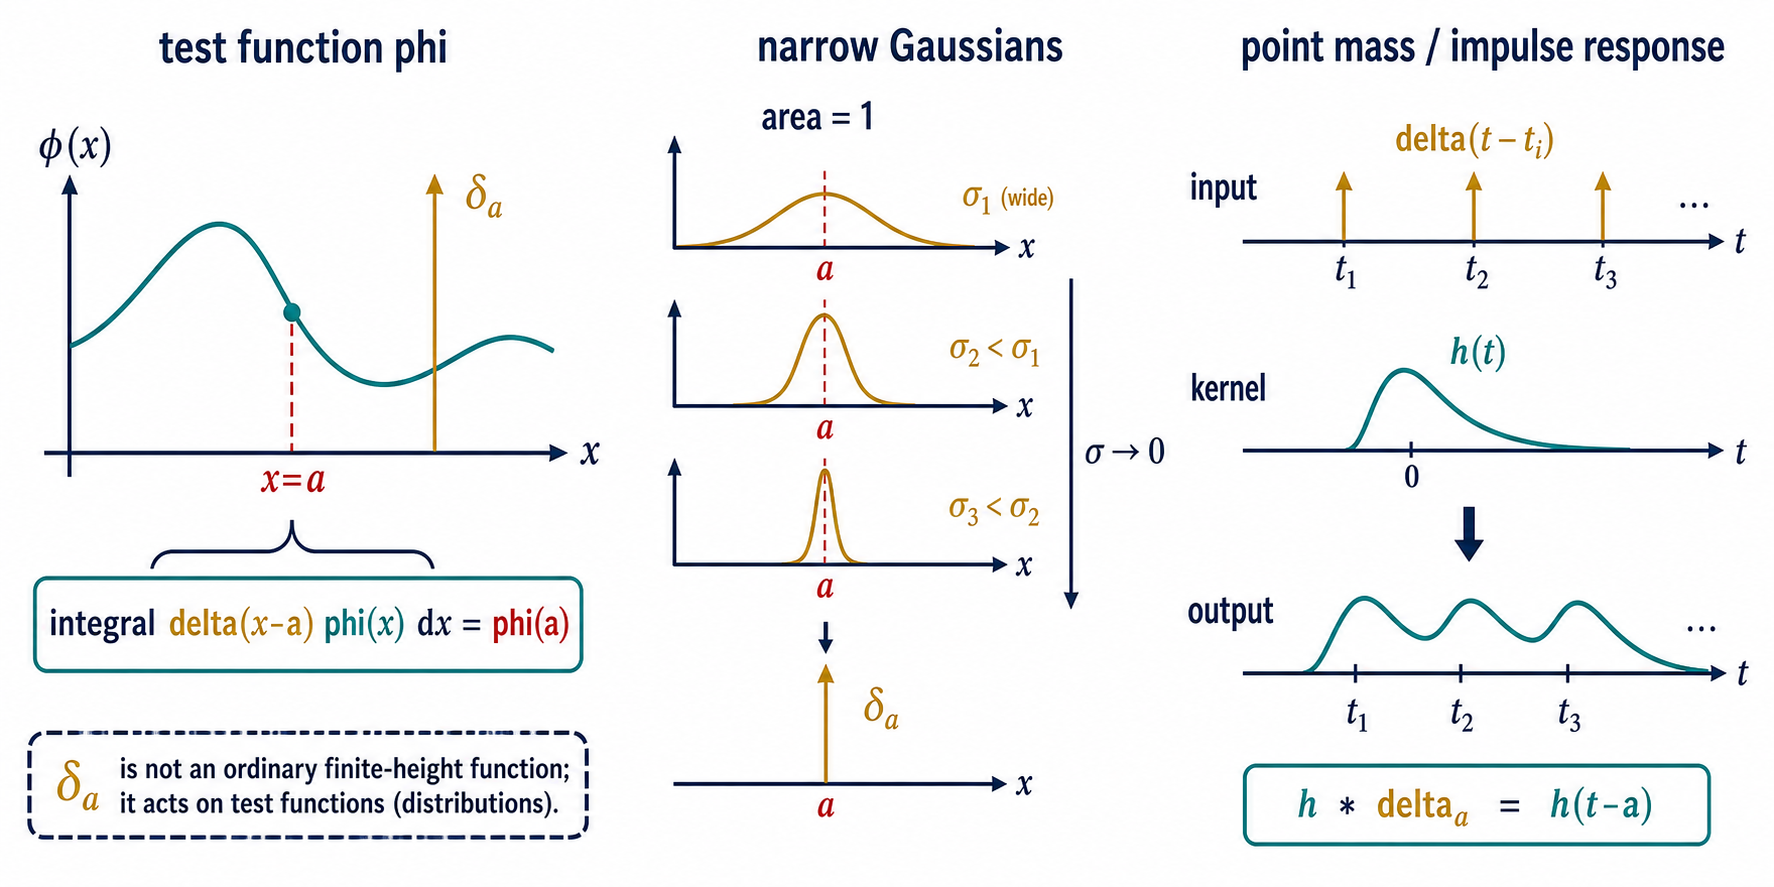
\includegraphics[width=0.98\linewidth]{imagegen-figures/ch11-delta-generalized-functions.png}
\caption{The Dirac delta acts on a test function by evaluation: \(\int \delta(x-a)\varphi(x)\,dx=\varphi(a)\). It can be approached by narrow unit-area bumps, and in signal models it represents an ideal impulse whose convolution with a kernel shifts the kernel to the impulse time.}
\label{fig:ch11-delta-generalized-functions}
\end{figure}

\paragraph{Formal setup.}
Let \(a\in\mathbb{R}\). The \emph{Dirac measure} at \(a\) is the probability measure \(\delta_a\) defined by
\[
\delta_a(A)=\mathbf{1}_A(a).
\]
If \(\varphi:\mathbb{R}\to\mathbb{R}\) is bounded and measurable, integration with respect to this measure gives
\[
\int \varphi(x)\,d\delta_a(x)=\varphi(a).
\]
The common notation
\[
\int \delta(x-a)\varphi(x)\,dx=\varphi(a)
\]
uses \(\delta(x-a)\) as if it were a density, but this is shorthand for integration with respect to the Dirac measure when \(\varphi\) is an ordinary measurable function. In distribution theory, the same symbol is used for a related action on smooth compactly supported test functions.

A \emph{generalized function} or \emph{distribution} is a linear rule that acts on smooth compactly supported test functions, written \(\varphi\in C_c^\infty(\mathbb{R})\). The Dirac delta acts by point evaluation:
\[
\langle \delta_a,\varphi\rangle=\varphi(a).
\]
The derivative of a distribution is defined for smooth test functions by moving the derivative onto the test function with a minus sign:
\[
\langle \delta_a',\varphi\rangle=-\langle \delta_a,\varphi'\rangle=-\varphi'(a),
\qquad \varphi\in C_c^\infty(\mathbb{R}).
\]
This definition is useful because it lets us differentiate objects that are not ordinary differentiable functions.

For a suitable kernel \(h\), convolution with a delta shifts the kernel:
\[
(h*\delta_a)(t)=h(t-a).
\]

\paragraph{Core intuition.}
Figure~\ref{fig:ch11-delta-generalized-functions} shows three compatible views. First, the delta evaluates a smooth test function at a point. Second, it can be approached by a sequence of narrow bumps whose total area remains one. Third, it acts as an ideal impulse in time: a spike at time \(a\) fed through a linear filter \(h\) produces the shifted response \(h(t-a)\).

The phrase "infinite at a point and zero elsewhere" is a tempting shortcut, but it is not a definition. A single point has zero ordinary length, so no finite-height density can assign positive probability to it. The correct rule is the integral action. The narrow-Gaussian picture is an intuition for convergence under integrals against smooth test functions, not pointwise convergence to an ordinary function.

A common misconception is that every probability distribution has a density \(p(x)\) with respect to \(dx\). Discrete distributions do not. Mixed distributions may have both atoms and continuous parts:
\[
P=0.2\,\delta_0+0.8\,p(x)\,dx.
\]
Here \(p\) is a normalized density, so \(\int p(x)\,dx=1\), and \(p(x)\,dx\) denotes the absolutely continuous measure \(A\mapsto\int_A p(x)\,dx\). The displayed expression is a weighted sum of measures, not an ordinary pointwise sum of functions. Measure theory lets these live in one language.

This section prepares Chapter 13's distinction between random variables and distributions, Chapter 14's discrete-continuous catalog, and later spike-train models where neural events are naturally represented as sums of deltas.

\paragraph{Main derivation: narrow Gaussians converge to the delta in action.}
Define the Gaussian bump
\[
\rho_\sigma(x)=\frac{1}{\sqrt{2\pi}\sigma}
\exp\!\left(-\frac{x^2}{2\sigma^2}\right),
\qquad \sigma>0.
\]
It is nonnegative and normalized:
\[
\int_{-\infty}^{\infty}\rho_\sigma(x)\,dx=1.
\]
For a bounded continuous test function \(\varphi\), and in particular for \(\varphi\in C_c^\infty(\mathbb{R})\), consider
\[
\int_{-\infty}^{\infty}\rho_\sigma(x-a)\varphi(x)\,dx.
\]
As \(\sigma\to0\), the mass of \(\rho_\sigma(x-a)\) concentrates near \(a\). Near \(a\), continuity gives \(\varphi(x)\approx\varphi(a)\). Therefore the integral behaves like
\[
\varphi(a)\int \rho_\sigma(x-a)\,dx=\varphi(a).
\]
The limiting statement is
\[
\lim_{\sigma\to0}\int \rho_\sigma(x-a)\varphi(x)\,dx
=
\varphi(a)
=
\langle\delta_a,\varphi\rangle.
\]
This is convergence as generalized functions: the objects converge by how they act under integrals, not by ordinary pointwise convergence.

For convolution, use the delta action directly:
\[
(h*\delta_a)(t)
=
\int h(t-s)\,d\delta_a(s)
=
h(t-a).
\]
The delta selects the value of the shifted kernel at \(s=a\).

\paragraph{Worked examples.}
\emph{Small symbolic example.} Let \(\varphi(x)=\sin x+x^2\). Then
\[
\int \delta(x-\pi)\varphi(x)\,dx
=
\varphi(\pi)
=
\sin\pi+\pi^2
=
\pi^2.
\]
If \(P=0.3\,\delta_0+0.7\,\delta_1\), then
\[
\mathbb{E}[X]=0.3(0)+0.7(1)=0.7.
\]
This expectation is an integral with respect to a discrete measure, not an integral against a continuous density.

\emph{ML/neuroscience example.} A spike train can be idealized as
\[
s(t)=\sum_{i=1}^n \delta(t-t_i),
\]
where \(t_i\) are spike times. Passing the spike train through a postsynaptic or smoothing kernel \(h\) gives
\[
(h*s)(t)=\sum_{i=1}^n h(t-t_i).
\]
The mathematical objects map directly to the neuroscience objects: each \(\delta(t-t_i)\) is an ideal spike event, \(h\) is the impulse response or smoothing kernel, and the convolution is the predicted filtered signal or firing-rate estimate.

\paragraph{ML/DL/neuroscience connections.}
In empirical risk minimization, the empirical data distribution is a sum of point masses:
\[
\widehat{P}_n=\frac{1}{n}\sum_{i=1}^n\delta_{x_i}.
\]
Expected loss under \(\widehat{P}_n\) becomes the sample average
\[
\int \ell(\theta,x)\,d\widehat{P}_n(x)
=
\frac{1}{n}\sum_{i=1}^n\ell(\theta,x_i).
\]
In differentiable signal models, deltas represent impulses, spike times, or idealized event inputs. In probabilistic modeling, atoms and continuous densities can be combined, which is essential for dropout-like masks, zero-inflated count models, and distributions with exact failure or threshold events.

\paragraph{Exercises.}
\begin{enumerate}[label=\textbf{11.4.\arabic*.}, leftmargin=*]
\item \textbf{Mechanical.} Compute \(\int \delta(x-3)(2x+1)\,dx\).
\item \textbf{Proof or derivation.} Use the definition \(\int \varphi\,d\delta_a=\varphi(a)\) to prove \((h*\delta_a)(t)=h(t-a)\).
\item \textbf{Numerical/computational.} Let \(\rho_\sigma(x)\) be the normalized Gaussian bump from the section. For \(\sigma=1,0.5,0.1\), describe what happens to its height and width while its total area remains \(1\).
\item \textbf{Interpretation.} Explain why the empirical distribution \(\widehat{P}_n=(1/n)\sum_i\delta_{x_i}\) turns expected loss into an average over training examples.
\item \textbf{Debug the misconception.} A student says, "The delta function must be an ordinary function with a very large value at one point." Explain why the test-function rule is the safer definition.
\end{enumerate}

\paragraph{Closing bridge.}
This chapter supplies the continuous bookkeeping that probability needs. Chapter 12 will also reuse integration and almost-everywhere equality to build \(L^2\) function spaces, where functions differing only on null sets are treated as the same object. Chapter 13 will turn probability into a measure \(P\) on a measurable space and define random variables as measurable functions. Chapters 14-15 will reuse densities, atoms, expectations, and marginalization to build distribution families and Bayesian updates. Later, change of variables will become the likelihood formula for normalizing flows, and delta functions will reappear in empirical distributions, spike trains, impulse responses, and generalized models of signals.

\clearpage
